\section{Introduction}\label{sec:promasens:introduction}
%
%Driven by the aim of building robots that can safely interact with complex and fragile environments,
%
% The past decade has seen an explosion of novel continuum soft robotic platforms \citep{luong2019eversion,shah2021soft,hughes2020extensible}. Inspired by invertebrate animals, these robots are almost entirely composed of soft deformable materials \citep{della2021soft}. This makes them robust and safe, but at the same time, it renders their modeling \citep{armanini2023soft}, control \citep{della2023model}, and shape sensing \citep{wang2018toward} substantially more complex than for their rigid counterparts.
%
\dropcap{S}hape sensing for continuum soft robots is especially complex because it is both a technological and algorithmic challenge. Rigid sensors must not obstruct the natural behavior or reduce the compliance of soft robots. At the same time, non-collocated and nonlinear sensors require algorithms for the measurements to be interpreted and connected to a description of the robot's shape.

Several sensing modalities have been considered to implement shape sensing, such as resistive~\citep{shih2019design, kramer2011soft}, capacitive~\citep{scimeca2019model, shintake2018ultrastretchable}, optical~\citep{li2021scaling}, and visual~\citep{rosi2022sensing}. Magnetic sensors~\citep{song2015electromagnetic, ozel2015precise, luo2017toward, guo2019continuum, mitchell2021fast} are a promising solution. Magnetic sensors are compact, highly sensitive, and can be easily integrated into existing soft robot designs. Thus, they can provide reliable and fully proprioceptive measurements at the cost of a minimal decrease in the robot's softness. Among the above-cited papers, the only work leveraging external magnetic fields is by \citet{song2015electromagnetic}, where coils placed at a distance generate the magnetic field.
Along these lines, an obvious choice would be to measure the Earth's magnetic field for proprioception purposes. However, it would only allow for the estimation of two rotational components, and any translational effects, such as an elongation of the continuum robot, could not be captured.
%\textcolor{blue}{Since a soft robot will elongate when pneumatically actuated, it is required to quantify the lengthening or shortening of the robot. This can not be achieved with solely an constant external magnetic source (like earth) and thus, an permanent magnet needs to be embedded in the robot.} 
Alternatively, some papers \citep{ozel2015precise,luo2017toward,guo2019continuum} use coaxial pairs of magnets and sensors embedded in the robot to estimate planar deformations. Recently, \citet{mitchell2021fast} has shown that a similar strategy can sense 3D deformations. Such simple arrangements greatly simplify the analysis, allowing for connecting readings to shape through direct interpolation. Nevertheless, relying on isolated pairs of sensors and magnets also strongly limits the density and the amount of information gathered through this method.

\begin{figure*}[ht]
  \centering
  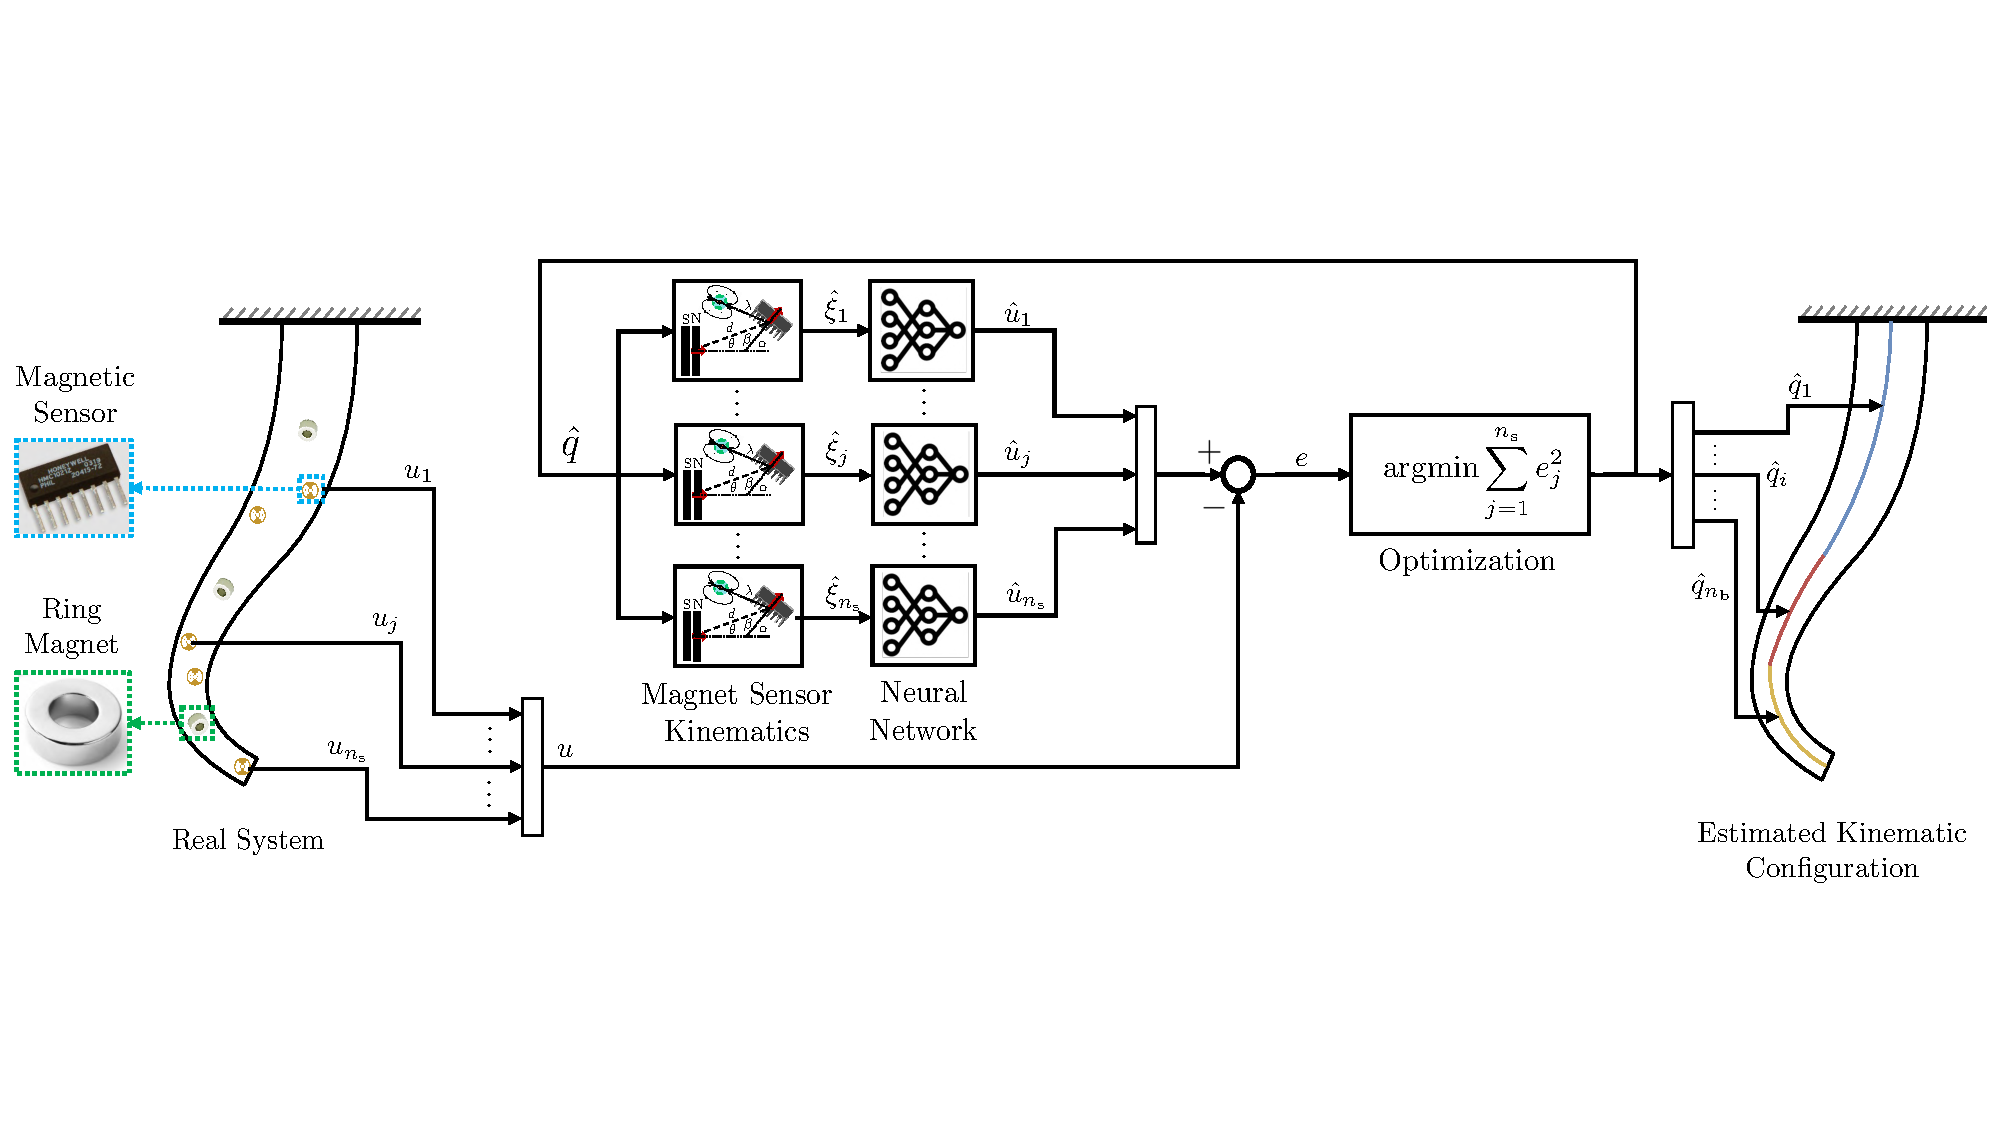
\includegraphics[width=1.0\textwidth]{promasens/figures/methodology/methodology_proprioception_v8_compressed.pdf}
  \caption{Proprioception for continuum soft robots with magnetic sensors: an initial configuration estimate $\hat{q}$ is employed to derive the kinematic relationship $\hat{\xi}$ between a sensor and each magnet. Subsequently, this kinematic description is used to predict the sensor measurements $\hat{u} \in \mathbb{R}^{n_\mathrm{s}}$ with a neural network trained in advance. A \gls{MSE} metric evaluates the accuracy of the predictions $\hat{u}$ compared to the actual measurements $u$. Finally, we optimize the configuration estimate $\hat{q}$ to achieve proprioception by minimizing the sensor measurement prediction loss.}\label{fig:promasens:methodology}
\end{figure*}

% However, the physical interaction between magnets, sensors, the earth's magnetic field and external disturbances is very complex and highly nonlinear.

% This means that simplified analytical models are usually not sufficient~\citep{ozel2015precise} and inverting the magnetic field equations directly to match sensor measurements with relative locations of the magnet and sensor is intractable~\citep{mitchell2021fast}.

% Related research published by \citet{guo2019continuum} consider a continuum robot made-up of many small sections each containing a magnet and a magnetic sensor. Their approach relies on an analytical model to estimate the 1D bending of small sections of a continuum robot. Subsequently, they fit Quadratic Bézier curves to the curvature of each section to model the shape of the continuum robot.

% An alternative to inaccurate analytical models is to conduct FEA simulations of the magnetic field for the chosen robot design and sensor layout~\citep{ozel2015precise, mitchell2021fast}.

% \citet{ozel2015precise} leverage Hall effect sensors to measure the curvature of a soft snake-like robot in 2D with both the sensor and magnet directly embedded in the silicon. They rely on data from FEA simulations stored in a look-up table to connect the measured magnetic flux density to translations relative to the magnet. A calibration function derived with least-squares fitting connects the relative translations to the soft robot curvature.

% Along a similar line of work, \citet{mitchell2021fast} follow a probabilistic approach by implementing a particle filter for proprioception with a tri-axis Hall effect sensor. The likelihood weight of each particle is given by the proximity of simulated magnetic flux measurements to the actual measurements.

% All existing approaches rely either on simplified analytical models, which are not suitable for complex geometric arrangements between magnets and sensors, or require to mirror the robot design with all necessary (DoF) in a simulator.

This chapter proposes to use permanent ring magnets and multiple magnetic sensors for shape sensing of continuum soft robots. Importantly, we remove the requirement of magnets and sensors being placed in coaxial pairs.
% placed at arbitrary locations within the soft segment. We then present a data-driven approach for making sense of the complex relationship between  measurements - so achieving proprioception with magnetic sensors.
%
We have been inspired by recent work leveraging deep learning to interpret various types of non-magnetic sensor data for proprioception purposes~\citep{truby2020distributed, ding2021predictive, soter2018bodily, thuruthel2019soft}.
% All of them except one~\citep{ding2021predictive} choose Recurrent Neural Network (RNN) structures as their neural network architecture to encourage temporal consistency of the robots' state estimates.
%
However, learning end-to-end mappings from sensors to configurations has three significant drawbacks: (i) it is data-intensive, (ii) it calls for recurrent architectures to encourage temporal consistency for the robot's configuration estimates, and (iii) it requires re-training when changing the kinematic model of the robot. We propose a neural architecture that circumvents all three issues (see Fig. \ref{fig:promasens:methodology}).
First, we train shallow neural networks to predict the measurements of the magnetic sensors from a parameterization describing their relative pose with respect to the magnets. We then optimize the configuration estimate - and thus the sensor positions - to minimize the error between the predicted and actual sensor measurements. 
% The result is the robot configuration estimate that better explains the sensor readings. 
This way, we introduce a priori information on the modes of deformation of a continuum soft robot, effectively removing the kinematics from the black box. 
The presented strategy enables us to re-arrange and remove redundant sensors during inference without requiring us to re-train the neural network on the adjusted sensor configuration.
% We provide experiments showing that this architecture achieves a mean precision of \SI{95.5}{\percent} when applied to 3D shape proprioception of a soft segment. 
% Testing on a similar trajectory type as trained on, even an error as low as \SI{1.4}{\percent} is possible.

% However, these existing solutions have some possible drawbacks~\citep{wang2018toward}. The piezoresistive and optical sensors are based over the entire length of the robot. This might result into issues with the robustness of these sensors when the robot has to deform more than the stretchability of the sensors allow. This issue could be resolved with Hall effect sensors, since there is no physical connection between the magnet and the sensor that restricts the robots motion. However, previous papers exploring the use of Hall effect sensors did not consider the estimation of 3D state parametrization.
% %
% This chapter proposes a kinematically decoupled, data-driven approach for achieving proprioception with magnetic sensors. We assume the placement of a permanent magnet at the center and multiple magnetoresistive sensors at arbitrary locations within the soft segment.
% Subsequently, we model the kinematic relationship between each magnet and sensor.
% This allows us to remove the kinematics from the black-box and train a neural network to predict the sensor measurements based on a very flexible input description independent of the used state parametrization of the robot.
% An advantage of this explicit kinematic description is that the position of a sensor or magnet can be changed without re-training the entire black-box if the neural network is trained on a sufficient large dataset of kinematic descriptions.
% We employ a loss between the predicted and actual sensor measurements to guide a nonlinear optimization strategy to compute the robot configuration estimate.
% The optimization approach consists of grid search running at lower frequencies in parallel to a fast gradient descent algorithm for local corrections.

% \textcolor{orange}{Do we hypothesize that this reduces the number of trainable parameters?}

% This chapter will explore the option to use \gls{MRS} and a permanent magnet, to find a relation between the \gls{MRS} output ans the sensor's position relative to the magnet. Due to the non-linearity of magnetic fields, it is hard to predict this relationship as found in previous 2D applications of similar sensors. Therefore, this chapter will look at using \gls{AI} to experimentally link the \gls{MRS} output to a 3D position.
%
% First, a model is needed that captures the position and movement of the robot. For this robot, the \gls{PCC} model is used~\citep{della2020improved}. Subsequently, this model can be used to find the parameters that physically relate the relative position of the magnet and the sensor, the \gls{MSK}. This will be used in combination with a \gls{NN} to predict the sensory output of a single sensor. Afterwards, the error between the predicted sensor output and the measured output is taken. By introducing multiple sensors, a gradient descent can be implemented to descent to the robots configuration by minimizing the error between the predicted and measured sensor values.

To summarize, this chapter contributes to the state of the art in soft robot sensing with:
%
\begin{itemize}
    \item A proprioceptive sensing modality relying on multiple magnetic sensors in conjunction with a neural network-based architecture that learns to estimate the full 3D shape of the robot from the sensor readings. % The strategy can deal with small training sets thanks to the injection of kinematic priors.
    % \item A data-driven approach to predict the measurements of \glsp{MRS} integrated into a multi-segment soft robot.
    \item Injection of kinematic priors through a description to spatially relate the poses of a sensor to the magnets. This proposed description serves as input to a neural network that predicts sensor measurements. %This kinematic description can be easily derived from the \gls{PCC} state description by providing the initial position of magnets and sensors in a straight robot configuration.
    % \item An optimization routine for minimizing the sensor prediction error by running a slow grid search and fast gradient descent in parallel.
    \item Experimental verification of the approach for a one-segment robot with three integrated \glspl{MRS} and proprioception of 3D curvature.    % \item A robust data-driven approach to achieve proprioception for a multi-segment, soft, snake-like robot in 3D.
    %\item Variable and scalable approach to \gls{MRS} measurements.
    % \item Combination of a data-driven sensor measurement model and \gls{MSK} in a gradient descent approach for proprioception.
    % \item Proposing a design how permanent magnets and \glsp{MRS} can be easily integrated into a soft robot.
\end{itemize}
We open-source a Python/PyTorch implementation of the proposed algorithm and the corresponding datasets on GitHub~\footnote{\url{https://www.github.com/tud-phi/promasens}}.
